\documentclass[12pt]{article}

\usepackage{float}
\usepackage{wrapfig}
\usepackage{geometry}
\usepackage{amsmath}
\usepackage{caption}
\usepackage{amssymb}
\usepackage{fancyhdr}
\usepackage{graphicx}
\usepackage{subcaption}

\pagestyle{fancy}
\setlength{\headheight}{20pt}

\lhead{5615 Assignment 1}
\chead{Alex Keating}
\rhead{March 05\textsuperscript{th}, 2019}

\begin{document}

\subsection*{CPU vs. GPU times}
    Between the three functions written, as was expected, in the serial version of the code the row sum function runs faster than the column sum function as the matrices are written in row major format and so the data is contiguous for the row sum function, this more efficient. Naturally, the reduce function runs much faster than both of these as it has only to do $\mathcal{O}(N)$ operations as opposed to $\mathcal{O}(N\times M)$ seen in the earlier two functions. These times can be seen in an example output screenshot seen in Figure \ref{fig:rowout}.\\
    \begin{figure}
        \centering
        \begin{subfigure}{0.48\textwidth}
            \centering
            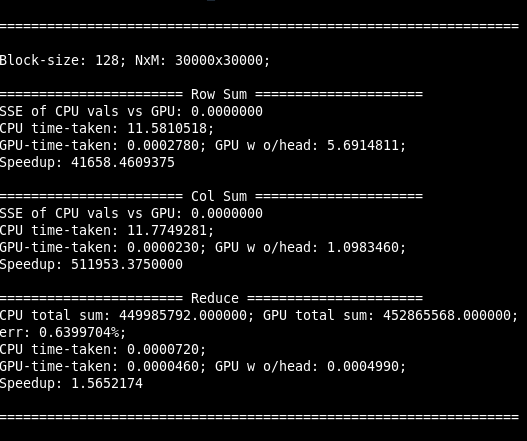
\includegraphics[width=0.75\linewidth]{rowScreen.png}
            \caption{Screnshot of example output with row sum first.}
            \label{fig:rowout}
        \end{subfigure}
        \begin{subfigure}{0.48\textwidth}
            \centering
            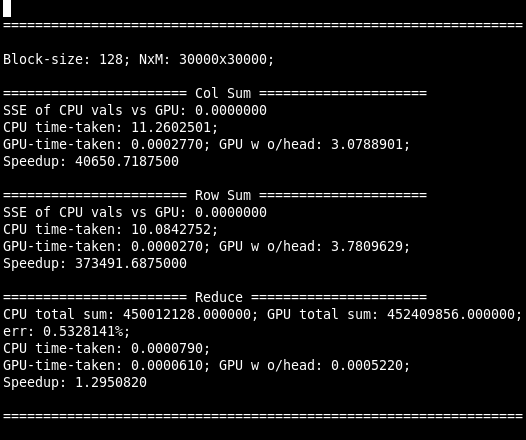
\includegraphics[width=0.75\linewidth]{colScreen.png}
            \caption{Screenshot of example output with column sum first.}
            \label{fig:colout}
        \end{subfigure}
        \caption{Example output screenshots.}
    \end{figure}
    The GPU times, on the other hand, did not perform quite exactly as expected. One would expect the times for the row-sum to be faster than the column sum in the GPU's case also, however, they actually performed slower. This was tested and did not appear to be related to the algorithm but actually moreso related to whichever function was run first. Figure \ref{fig:colout} shows anoterh output screenshot where the column sum function was ran first. It can be seen to run slower this time, implying that this is possibly due to some hardware problem of the GPU needing to "warm-up" for lack of a better term.
    \begin{figure}
        \centering
        \begin{subfigure}{0.48\textwidth}
            \centering
            \includegraphics[width=\linewidth]{../plots/logRowSpeedup}
            \caption{Log scale of speedupds for row sum.}
            \label{fig:rowSU}
        \end{subfigure}
        \begin{subfigure}{0.48\textwidth}
            \centering
            \includegraphics[width=\linewidth]{../plots/logColSpeedup}
            \caption{Log scale of speedupds for column sum.}
            \label{fig:colSU}
        \end{subfigure}\\ %%
        \begin{subfigure}{0.32\textwidth}
            \centering
            \includegraphics[width=\linewidth]{../plots/logRedSpeedup}
            \caption{Log scale of speedupds for reduce.}
            \label{fig:redSU}
        \end{subfigure}
        \begin{subfigure}{0.32\textwidth}
            \centering
            \includegraphics[width=\linewidth]{../plots/absRedSpeedup}
            \caption{Absolute value of speedups for reduce.}
            \label{fig:redabsSU}
        \end{subfigure}
        \begin{subfigure}{0.32\textwidth}
            \centering
            \includegraphics[width=\linewidth]{../plots/logRedSpeedup}
            \caption{Absolute times of reduce for CPU \& GPU.}
            \label{fig:GPUvsCPU}
        \end{subfigure}
        \caption{Function speedups of GPU vs. CPU.}
        \label{fig:SU}
    \end{figure}
    Thankfully, the speedups seen did behave as one would expect. However, the difference in speedup between the row sum and column sum functions can be taken with a grain of salt as by interchanging the order within which they are executed will effectively swap their speedup times. Figure \ref{fig:SU} shows the substantial speedups seen in the first two functions getting up to orders of $10^6\times$. As the size of the problem increases the speedup also as expected increases. The reduce function only actually appears to see speedups at $N\times M$ reaching $30,000\times30,000$, presumably due to the need for multiple thread synchronisations compared to the one sync in the othe other two functions. 
    \begin{figure}
        \centering
        \begin{subfigure}{0.32\textwidth}
            \centering
            \includegraphics[width=\linewidth]{../plots/absRowTime}
            \caption{Absolute times for row sum.}
            \label{fig:rowabs}
        \end{subfigure}
        \begin{subfigure}{0.32\textwidth}
            \centering
            \includegraphics[width=\linewidth]{../plots/absColTimes}
            \caption{Absolute times for column sum.}
            \label{fig:colabs}
        \end{subfigure}
        \begin{subfigure}{0.32\textwidth}
            \centering
            \includegraphics[width=\linewidth]{../plots/absRedTimes}
            \caption{Absolute times for reduce.}
            \label{fig:redabs}
        \end{subfigure}
        \caption{Absolute times take on GPU.}
        \label{fig:abs}
    \end{figure}
    Figure \ref{fig:abs} shows the absolute times of the GPU execution of each function for each of the matrix sizes, versus the block size in number-of-threads. It is not clear from any of those results nor from the speedups that there is any evident optimal block size for this problem, and so this ended up being inconclusive. The absolute times taken for the GPU are seen to be quite erratic and no real pattern can be seen in them. Rather strangely, in some of the case that can be seen, the larger problem size takes less time than the smaller.  

\subsection*{Errors}
    \begin{wrapfigure}{r}{0.5\textwidth}
        \centering
         \includegraphics[width=\linewidth]{../plots/percErrRed}
         \caption{Percentage error between CPU and GPU final values for reduce.}
         \label{fig:err}
    \end{wrapfigure}
    In order to evaluate the accuracy of the software, an SSE calculation was performed on the resulting vectors from the row sum and column sum functions between the CPU returned values and GPU returned values. In all cases, the resulting SSE was $0.0$ to 7 decimal places. The reduce function, a percentage difference was found between the CPU and GPU returned values. In most cases, barring in Figure \ref{fig:err} showing 3 outliers, all errors were of the order of $\sim10^{-5}$ percent. However, again in the accuracy tests, it does not appear clear that there is any evident optimal choice of block size.

\subsection*{Doubles vs. Floats}
    Again. some erratic results were received for some of the tests in this program. One would expect that the time taken to process floats on the GPU would run universally slower than processing float. However, as can be seen in Figure \ref{fig:dbl}, there is no consistent result to say that doubles run slower than floats for any block size of matrix size.
    \begin{figure}
        \centering
        \begin{subfigure}{0.32\textwidth}
            \centering
            \includegraphics[width=\linewidth]{../plots/rowDblFl}
            \caption{Row sum float time - double time.}
            \label{fig:rowdbl}
        \end{subfigure}
        \begin{subfigure}{0.32\textwidth}
            \centering
            \includegraphics[width=\linewidth]{../plots/colDblFl}
            \caption{Column sum float time - double time.}
            \label{fig:coldbl}
        \end{subfigure}
        \begin{subfigure}{0.32\textwidth}
            \centering
            \includegraphics[width=\linewidth]{../plots/redDblFl}
            \caption{Row sum float time - double time.}
            \label{fig:reddbl}
        \end{subfigure}
        \caption{Difference in time taken using floats or doubles.}
        \label{fig:dbl}
    \end{figure}

\end{document}
